%!TEX root = ../thesis.tex
\chapter{Evaluation}\label{evaluation}


\ifpdf
    \graphicspath{{Chapter3/Figs/Raster/}{Chapter3/Figs/PDF/}{Chapter3/Figs/}}
\else
    \graphicspath{{Chapter3/Figs/Vector/}{Chapter3/Figs/}}
\fi


\NOTE{A}{I am really not sure about the best structure for this chapter.}

\section{General Notes}

In this chapter I provide quantitative and qualitative analysis and comparison of the settings presented in previous chapters.


To obtain thorough and statistically significant results, I utilised parallel processing as much as possible for evaluating Deep Q-Learning policies, which are the bottleneck of the evaluation phase. To exploit the parallelism of the GPU even with the inherently sequential MDP, I ran several (usually $64$) independent samples in parallel. Note that this is much simpler for \textsc{Two-Thinning} and \textsc{Graphical Two Choice}, where the number of steps from start to end in the MDP is constant ($m$) in any execution.


Even with this evaluation speedup, the usability of Deep Q-Learning for large values of $n$ and $m$ is still limited due to the training time. The largest range for which I successfully trained a RL algorithm in at most a day is $n=1000$, $m=1500$, but I decided to focus on slightly smaller values for the evaluation as that is more illustrative and complementary to the literature available.



\NOTE{A}{TODO: Note that in this project there is no train or test set, there isn’t any data at all. Nevertheless, it is still important to do evaluation independently of early stopping, due to the Expectation-Maximum Jensen inequality.}


\section{Two-Thinning}


\subsection{Comparison of Strategies}

Now I present a comparison of seven \textsc{Two-Thinning} strategies. I have chosen nine combinations of $n$ (number of bins) and $m$ (number of balls) so that they cover different ranges, and also different balls-bins ratios.


To have acceptable statistical significance but also reasonable runtime, I compared the strategies across $100$ runs. I show the average of scores (maximum load) of the runs and also the $95\%$ confidence interval for the estimated mean score, based on the Central Limit Theorem (CLT). \NOTE{A}{Should I explain more? Any formal statistical reason for choosing the number of runs?}


Note that the Dynamic Programming (DP) Strategy is optimal by definition, but it is too slow for larger values of $n$ and $m$ which I denote by TLE (Time Limit Exceeded). I decided to limit all the algorithms to $12$ hours of training/preparation, declaring anything above that as TLE. Also, even though we have the exact expected maximum load of the DP Strategy, I decided to run it just like the other strategies for fair comparison (e.g. large outliers that the DP Strategy takes into account occur very rarely during execution).


For the Threshold Strategy, I calculated the optimal values by modelling it as a Multi-Armed Bandit problem (covered in II Randomised Algorithms) \cite{katehakis1987multiarmedbandit}, and using an $\epsilon$-greedy strategy with $\epsilon=0.1$ (details omitted).


I note that there is merit in not just doing several runs with the trained trained Deep Q-Learning model, but also retraining it several times (e.g. $20$ runs with each of $5$ independently trained model), because the rewards received during training are also probabilistic. This idea would rather evaluate the robustness of the Deep Q-Learning framework for balls into bins settings, but I decided to stick to a single trained model and essentially evaluate the peak performance. \NOTE{A}{Does it make any sense? This idea came to my mind and I am a bit unsure about it and couldn't find any reference.}. Relatedly, one could consider finding the optimal hyperparameters as a special part of training, but I decided treat it separately, and in particular, not take it into account for the $12$ hour TLE limit.


\begin{table}[h!]
\label{tab:two-thinning-comparison}
\centering
\resizebox{\textwidth}{!}{%
\begin{tabular}{|l|c|c|c|c|c|c|c|c|c|}
\hline
                                & \multicolumn{3}{c|}{$n=5$} & \multicolumn{3}{c|}{$n=20$} & \multicolumn{3}{c|}{$n=50$} \\ \hline
Strategy                                & $m=5$ & $m=10$ & $m=25$ & $m=20$ & $m=60$ & $m=400$ & $m=50$ & $m=200$ & $m=2500$ \\ \hline
Always Accept          & 2.26 $\pm$ 0.06 & 3.84 $\pm$ 0.1 & 7.88 $\pm$ 0.14 & 3.26 $\pm$ 0.1 & 6.68 $\pm$ 0.15 & 28.84 $\pm$ 0.32 & 3.87 $\pm$ 0.1 & 9.12 $\pm$ 0.16 & 66.66 $\pm$ 0.5 \\ \hline
Random             & 2.35 $\pm$ 0.07 & 3.72 $\pm$ 0.09 & 7.66 $\pm$ 0.14 & 3.21 $\pm$ 0.1 & 6.67 $\pm$ 0.15 & 28.55 $\pm$ 0.32 & 3.8 $\pm$ 0.1 & 9.02 $\pm$ 0.18 & 66.83 $\pm$ 0.48 \\ \hline
Local Reward Optimiser & 1.82 $\pm$ 0.05 & 2.97 $\pm$ 0.05 & 6.08 $\pm$ 0.06 & 2.25 $\pm$ 0.06 & 4.75 $\pm$ 0.08 & 22.46 $\pm$ 0.09 & 2.54 $\pm$ 0.07 & 6.37 $\pm$ 0.07 & 53.98 $\pm$ 0.11 \\ \hline
Mean Thinning          & 1.87 $\pm$ 0.07 & 3.1 $\pm$ 0.07 & 6.17 $\pm$ 0.09 & 2.56 $\pm$ 0.08 & 5.12 $\pm$ 0.1 & 22.52 $\pm$ 0.12 & 3.06 $\pm$ 0.08 & 6.79 $\pm$ 0.11 & 53.53 $\pm$ 0.15 \\ \hline
DP                   & 1.85 $\pm$ 0.06 & 2.98 $\pm$ 0.07 & 6.06 $\pm$ 0.1 & 2.33 $\pm$ 0.1 & 4.69 $\pm$ 0.11 & TLE & 2.52 $\pm$ 0.1 & TLE & TLE \\ \hline
Deep Q-Learning        & 1.92 $\pm$ 0.09 & 2.93 $\pm$ 0.09 & 6.2 $\pm$ 0.11 & 2.42 $\pm$ 0.1 & 4.88 $\pm$ 0.12 & 22.2 $\pm$ 0.14 & 2.5 $\pm$ 0.11 & 6.43 $\pm$ 0.11 & 53.49 $\pm$ 0.25 \\ \hline
Threshold           & 2.18 $\pm$ 0.13 & 3.32 $\pm$ 0.13 & 6.44 $\pm$ 0.13 & 2.58 $\pm$ 0.12 & 5.58 $\pm$ 0.17 & 24.12 $\pm$ 0.19 & 2.99 $\pm$ 0.12 & 7.02 $\pm$ 0.13 & 56.73 $\pm$ 0.29 \\ \hline 

\end{tabular}}
\caption{Average maximum load of \textsc{Two-Thinning} strategies with $95\%$ confidence intervals}
\end{table}


We can see that the Always Accept and Random Strategies are consistently poorly performing. The DP Strategy is not shown to be exactly the best for reasons outlined above. The Threshold Strategy, even though asymptotically shown to be optimal is outperformed by several other strategies. The difference is even more significant for larger $m$, when the constant threshold (on the primary allocations) is too much of a restriction. The Mean Thinning, Local Reward Optimiser and Deep Q-Learning Strategies seem to be comparable to each other. I have calculated the one-sided p-values of a two sample t-test to see if the Deep Q-Learning Strategy is significantly better than the Mean Thinning Strategy for larger values of $n$ and $m$. The difference is significant for most of the cases (the p-values are $\sim 10^{-3}$ for $n=20$, $m=400$, $\sim 10^{-17}$ for $n=50$, $m=50$, $\sim 10^{-5}$ for $n=50$, $m=200$) but more data would be required for $n=50$, $m=2500$. \NOTE{A}{Double check that I am not writing something stupid. In particular, the test I applied assumes that the maximum loads are from a normal distribution and the two distributions have the same variance and none of them are actually true, at least not exactly... How to remedy this?} \NOTE{A}{Should I do some more p-values or this is enough to convince them about the professionalism of this dissertation?}

\NOTE{A}{Should I say some more, clever bullshit about the table, some general patterns, etc.? Maybe a bit more about the difference between the columns, not between the rows.}


One of the main surprises of the comparison is that the Local Reward Optimiser Strategy (which rejects only the maximum loads) has similar performance as the Deep Q-Learning Strategy, which was trained to optimise cumulative rewards. This suggests that the RL problem underlying \textsc{Two-Thinning} is a challenging one, in particular, learning long-term consequences of decisions is difficult, because the impact of a single ball is very subtle. In general, making a small number of bad decisions might not even impact the final maximum load. \NOTE{A}{TODO: elaborate some more? This is a crucial point to make.}


\NOTE{A}{Write a bit about the running time of both training and evaluation. DQN would be a bit slower latency-wise but it is bearable. Note that other strategies require no training.}



\NOTE{A}{Add plot showing that it doesn't work very well for larger $n$ and $m$. Add general plots for huge $n$ and $m$. Also I can include here the tendencies for the theoretical results, e.g. plotting a logarithmic curve. Mention the difficulty in finding the constant factor of those theoretical algorithms.}



Analysing the optimal strategies for \textsc{Two-Thinning}, I formulated the following lemma.

\begin{lemma}\label{lemma: two-thinning-increasing-threshold}
The chosen thresholds of an optimal protocol are non-decreasing during an execution. That is, if for $i$th ball the protocol chooses a threshold $x$, then for every $j$th ball of the same game such that $j>i$, a threshold $y\geq x$ is chosen.
\end{lemma}


\begin{figure}[h!] \label{dp-increasing-threshold}
    \centering
    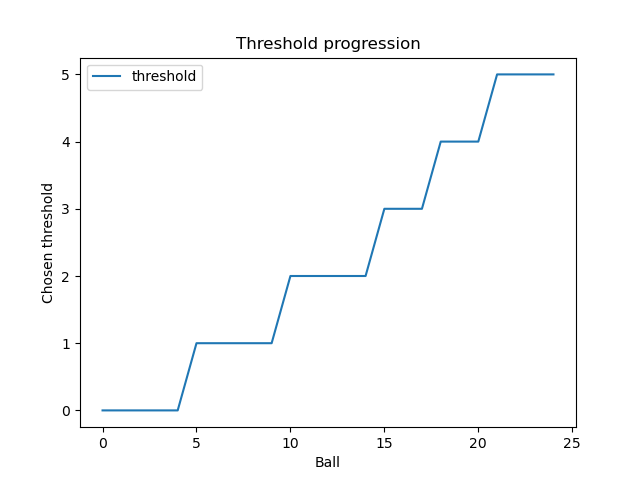
\includegraphics[scale=1.0]{Chapter4/Figs/dp_increasing_threshold.png}
    \caption{A run of the DP Strategy showing the increasing threshold property}
\end{figure}

This is a very surprising lemma, because the theoretically asymptotically optimal protocols in the literature do not have this property. We think that this is because they are optimal only up to a constant (or logarithmic) factor, and they are easier to reason about analytically and prove bounds on them (usually these protocols consist of independent phases with different behaviour).


\begin{proof}

\NOTE{A}{Do proper proof.}
\NOTE{T}{Do we really think we have a proof of that?}

The lemma has been verified by the optimal strategy(s) generated by dynamic programming, for several combinations of $n$ and $m$. 
\end{proof}


As discussed in Chapter \ref{preparation}, there are several other reasonable objective functions, such as maximising minimum load, minimising maximum load minus minimum load, minimising variance, and all of those that I have used as potential functions. I do not discuss this any further due to the length constraint on the dissertation, I just note that I found that it is very difficult for Deep Q-Learning to adapt its decisions on such a granular level. 


\subsection{Deep Q-Learning analysis}



\NOTE{A}{Maybe add an analysis of Threshold ``Spikes'' During Training and During Execution}



\subsubsection{Hyperparameter Analysis}

\NOTE{A}{Compare zero potential with max load potential, showing P value that we do need reward shaping.}


The Weights and Biases tool provides an analysis of the importance of hyperparameters. It calculates the correlation coefficient between the hyperparameters and the score for each hyperparameter (green is positive, red is negative). To capture interactions between hyperparameters and also non-linear relationships, it also provides an importance score which is calculated based on Random Forests \cite{biewald2020wandb}.


I present the hyperparameter importance analysis of $200$ runs for the $n=20$ and $m=40$ case, but the pattern is similar for other cases too.


\begin{figure}[h!] \label{two-thinning-hyperparameter-importance}
    \centering
    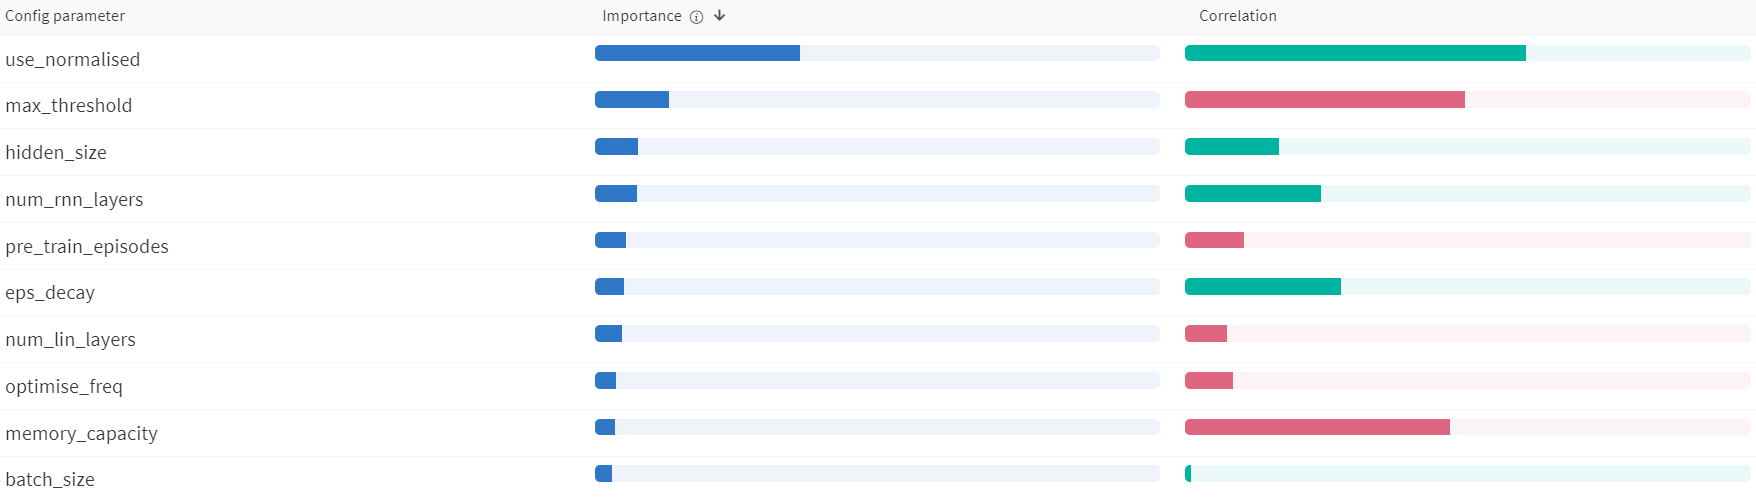
\includegraphics[scale=0.4]{Chapter4/Figs/Hyperparameter_importance_20_400.png}
    \caption{\textsc{Two-Thinning} Hyperparameter Importance}
\end{figure}


We can see that the most important hyperparameter is to use the normalised domain. As discussed earlier, this helps because in the normalised domain, a constant threshold is already a reasonable strategy (see e.g. Mean Thinning). Also, limiting the maximum threshold that the agent can use restricts the search space, and fosters learning. As can be seen in Appendix \ref{hyperparameters}, the ideal maximum threshold is around the target expected maximum load we want to achieve (which can be estimated based on theoretical results).



\subsubsection{Training}


\begin{figure}[h!] \label{two-thinning-training-curve}
    \centering
    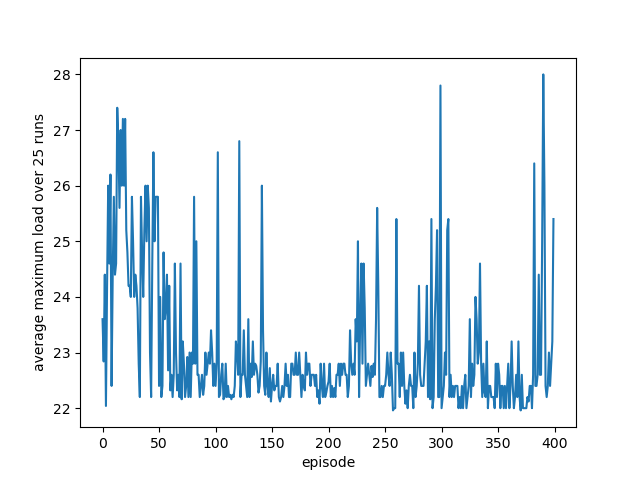
\includegraphics[scale=1.0]{Chapter4/Figs/training_progression_20_400.png}
    \caption{\textsc{Two-Thinning} Training Curve $n=20$, $m=400$}
\end{figure}


We can see that the improvement during training decays very quickly, and the agent is close to its best already at the start. This is again due to the normalised load domain outlined above - I plotted the training curve without the normalised load domain trick, and that shows a much more usual training progression, though leading to a worse optimum. The oscillations are due to both the inherent randomness in evaluation and the agent trying to change its policy in a wrong way.


Motivated by the fact that in the normalised domain, a constant $0$ threshold is the Mean Thinning Strategy, I tried to see if this simple strategy can be improved by choosing another constant ``offset'', not $0$.:

\begin{figure}[h!] \label{two-thinning-training-curve}
    \centering
    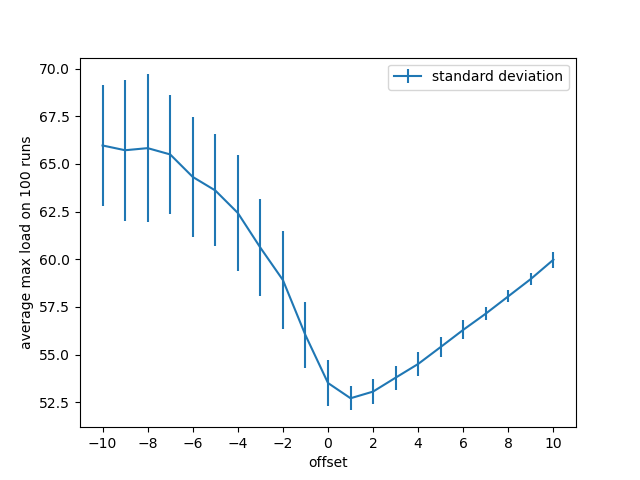
\includegraphics[scale=1.0]{Chapter4/Figs/offset_analysis_50_2500.png}
    \caption{Comparing constant offset strategies for $n=50$, $m=2500$}
\end{figure}


On the figure we can see that for $n=50$, $m=2500$, the best offset is $1$. It holds for general $n$ and $m$ that the best offset is usually slightly above $0$.

The Deep-Q Learning algorithm, which is as shown above, statistically significantly better than Mean-Thinning, actually often learns a strategy close to a constant offset strategy.


\begin{figure}[h!] \label{two-thinning-training-curve}
    \centering
    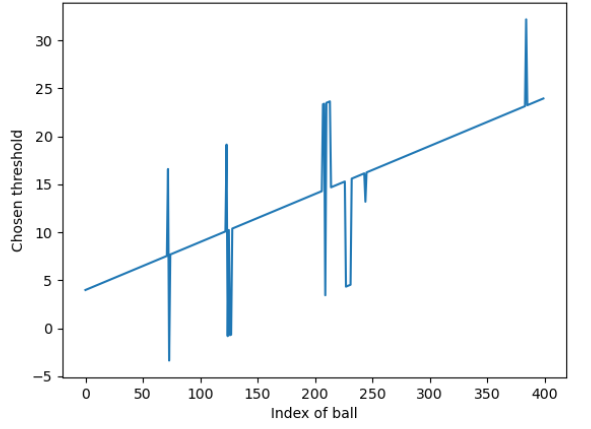
\includegraphics[scale=1.0]{Chapter4/Figs/dqn_learnt_thresholds.png}
    \caption{Analysis of the chosen thresholds of the Deep Q-Learning Strategy for $n=20$, $m=400$. Note that this plot shows only a single run, and the actual load vectors are not displayed.}
\end{figure}


The sporadic ``jumps'' are very challenging for the agent to get rid of, because as discussed above, a few bad decisions don't have strong impact on the result. To avoid this, as future work the agent could be constrained to change the threshold at most by $1$ after each ball (we have empirical evidence for this to hold for any optimal strategy).




\subsection{Distribution of the States Under an Optimal Strategy}

\NOTE{A}{we can observe an exponentially decreasing function!}
\NOTE{A}{Entropy is fairly low - this could be used as a speedup for RL training (or even as the curriculum for pretraining)}


\section{K-Thinning}



\subsection{Comparison of Strategies}


\NOTE{T}{make $k$ and $K$ more consistent}
\begin{table}[h!]
\label{tab:k-thinning-comparison}
\centering
\resizebox{\textwidth}{!}{%
\begin{tabular}{|l|c|c|c|c|c|c|c|c|}
\hline
                                & \multicolumn{4}{c|}{$n=5$} & \multicolumn{4}{c|}{$n=25$}\\ \hline
                                & \multicolumn{4}{c|}{$m=20$} & \multicolumn{4}{c|}{$m=50$}\\ \hline
Strategy                                & $k=2$ & $k=3$ & $k=5$ & $k=10$ & $k=2$ & $k=3$ & $k=5$ & $k=10$ \\ \hline
Always Accept           & 7.88 $\pm$ 0.14 & 7.72 $\pm$ 0.11 & 7.81 $\pm$ 0.14 & 7.8 $\pm$ 0.14 & 5.65 $\pm$ 0.19 & 5.81 $\pm$ 0.13 & 5.84 $\pm$ 0.14 & 6.03 $\pm$ 0.16 \\ \hline
Random                 & 7.66 $\pm$ 0.14 & 7.76 $\pm$ 0.13 & 7.77 $\pm$ 0.14 & 7.74 $\pm$ 0.14 & 5.77 $\pm$ 0.19 & 5.96 $\pm$ 0.15 & 5.87 $\pm$ 0.15 & 5.72 $\pm$ 0.14 \\ \hline
Local Reward Optimiser & 6.08 $\pm$ 0.06 & 5.77 $\pm$ 0.05 & 5.45 $\pm$ 0.06 & 5.13 $\pm$ 0.04 & 4.22 $\pm$ 0.11 & 3.69 $\pm$ 0.06 & 3.21 $\pm$ 0.06 & 3.0 $\pm$ 0.01 \\ \hline
DP & 6.06 $\pm$ 0.1   & 5.75 $\pm$ 0.05 & 5.38 $\pm$ 0.05 & 5.1 $\pm$ 0.03 & 4.13 $\pm$ 0.09 & 3.58 $\pm$ 0.07 & 3.15 $\pm$ 0.05 & 3.0 $\pm$ 0.0 \\ \hline Threshold              & 6.44 $\pm$ 0.13 & 6.27 $\pm$ 0.05 & 6.12 $\pm$ 0.05 & 5.93 $\pm$ 0.05 & 4.72 $\pm$ 0.15 & 4.17 $\pm$ 0.05 & 4.0 $\pm$ 0.05 & 3.94 $\pm$ 0.05 \\ \hline
Deep Q-Learning        & 6.2 $\pm$ 0.11 & 6.77 $\pm$ 0.11 & 7.14 $\pm$ 0.14 & 7.14 $\pm$ 0.14 & 4.26 $\pm$ 0.09 & 4.47 $\pm$ 0.09 & 4.21 $\pm$ 0.08 & 3.01 $\pm$ 0.01 \\ \hline 
Quantile          & 6.17 $\pm$ 0.09 & 5.96 $\pm$ 0.04 & 5.61 $\pm$ 0.06 & 5.15 $\pm$ 0.04 & 4.34 $\pm$ 0.12 & 3.69 $\pm$ 0.07 & 3.15 $\pm$ 0.05 & 3.0 $\pm$ 0.01 \\ \hline
\end{tabular}}

\caption{Average maximum load of \textsc{K-Thinning} strategies with $95\%$ confidence intervals}
\end{table}


\NOTE{A}{Analyse value of K and its impact.}

\begin{lemma} \label{lemma: k-thinning-increasing-threshold}
In an optimal strategy, it is not possible that it would accept a bin with $x$ choices left, but reject the same bin (with the same loads) with $y<x$ choices left. In other words, an optimal strategy should never become more selective after rejecting some options.
\end{lemma}


\begin{proof}
Note that Lemma \ref{lemma: thresholdproperty} generalises to \textsc{K-Thinning} as well - an optimal strategy must base its decisions on a threshold.


\NOTE{A}{TODO: add real proof}.


Using the dynamic programming algorithm, that creates the optimal strategy(s), I verified the lemma, that is that the threshold is indeed non-decreasing within the same load configuration.
\end{proof}


\subsection{Deep Q-Learning analysis}


\subsubsection{Training}


\subsubsection{Hyperparameter Analysis}



\section{Graphical Two-Choice}


\subsection{Comparison of Strategies}
\begin{table}[h!]
\label{tab:graphical-two-choice-comparison}
\centering
\resizebox{\textwidth}{!}{%
\begin{tabular}{|l|c|c|c|c|c|c|c|c|c|}
\hline
                                & \multicolumn{3}{c|}{$n=4$} & \multicolumn{3}{c|}{$n=16$} & \multicolumn{3}{c|}{$n=32$}\\ \hline
                                & \multicolumn{3}{c|}{$m=25$} & \multicolumn{3}{c|}{$m=50$} & \multicolumn{3}{c|}{$m=32$}\\ \hline
Strategy                                & Cycle & Hypercube & Complete & Cycle & Hypercube & Complete & Cycle & Hypercube & Complete \\ \hline
Greedy  & 7.04 $\pm$ 0.03 & 7.04 $\pm$ 0.03 & 7.17 $\pm$ 0.06 & 4.74 $\pm$ 0.08 & 4.47 $\pm$ 0.11 & 4.39 $\pm$ 0.07 & 2.46 $\pm$ 0.1 & 2.34 $\pm$ 0.09 & 2.26 $\pm$ 0.06 \\ \hline
Random  & 8.92 $\pm$ 0.17 & 8.81 $\pm$ 0.18 & 8.98 $\pm$ 0.17 & 6.75 $\pm$ 0.17 & 6.64 $\pm$ 0.23 & 6.56 $\pm$ 0.15 & 3.45 $\pm$ 0.13 & 3.64 $\pm$ 0.16 & 3.54 $\pm$ 0.1 \\ \hline
Local Reward Optimiser & 7.1 $\pm$ 0.04 & 7.12 $\pm$ 0.05 & 7.29 $\pm$ 0.07 & 4.97 $\pm$ 0.1 & 4.74 $\pm$ 0.12 & 4.75 $\pm$ 0.07 & 2.53 $\pm$ 0.11 & 2.42 $\pm$ 0.1 & 2.46 $\pm$ 0.07 \\ \hline
DP & 7.01 $\pm$ 0.02 & 7.01 $\pm$ 0.02 & 7.27 $\pm$ 0.1 & TLE & TLE & TLE & TLE & TLE & TLE \\ \hline
Deep Q-Learning & 7.17 $\pm$ 0.07 & 7.17 $\pm$ 0.06 & 7.38 $\pm$ 0.09 & 4.92 $\pm$ 0.15 & 5.71 $\pm$ 0.17 & 6.57 $\pm$ 0.15 & 3.81 $\pm$ 0.18 & 3.59 $\pm$ 0.18 & 4.17 $\pm$ 0.14 \\ \hline 

\end{tabular}}

\caption{Average maximum load of \textsc{Graphical Two Choice} strategies with $95\%$ confidence intervals\protect\footnotemark}
\end{table}

\footnotetext{Note that for $n=4$, Cycle and Hypercube are the same graphs.}

First I prove the most surprising result of this section.

\begin{lemma} \label{lemma: greedy-suboptimal}
There exist a graph, such that the Greedy strategy is suboptimal with respect to the expected final maximum load of \textsc{Graphical Two Choice}.
\end{lemma}

\begin{proof}
It is enough to show that there is a state $s$ (i.e. a load vector $v$, edge $e$) where is is better to choose the bin with the larger load. This suffices because there is a non-zero probability of reaching $s$, and hence a strategy which agree with Greedy everywhere else except for this state has a strictly better expected score.


I used the dynamic programming algorithm to find the optimal strategy for \textsc{Graphical Two Choice}, and then I searched the strategy for a state where it disagrees with Greedy. I found a very small counterexample for the Cycle graph with $n=4$ bins $m=6$ balls. Denoting the nodes as ($1$-based) indices in the load vector, the counterexample state is $l=(2,0,1,0)$, $e=(2,3)$, i.e. there is an edge between the second and third bin. The reason why it is better to choose bin $3$ even though it has larger load than bin $2$ is that after that, from load vector $(2,0,2,0)$ with $2$ balls remaining we can definitely avoid having a maximum load $3$ by always placing the ball in an even-indexed bin. On the other hand, from load vector $(2,1,1,0)$, if both of the remaining edges are $(1,2)$, then there will be a maximum load of at least $3$ using whatever strategy. Therefore, the expected final maximum load of choosing bin $3$ is $2.0$, while that of bin $2$ is between $2.0$ and $3.0$.
\end{proof}


We can see from the table, that for $n=4$ and $m=25$, even though Greedy is not optimal for the Cycle graph but it is for the Clique graph, the optimal strategy for the Cycle graph (provided by the DP Strategy) still has a lower expected maximum load than Greedy has for the Clique graph. This is an important observation, because it indicates that the constraint that not all the pairs of nodes can be sampled (e.g. due to geographical reasons) is not just a constraint, but it can even improve the performance in some special cases.


For larger graphs, however, Greedy tends to perform better on the Clique graph than on the others. Hypothesising that its performance depends on the sparsity of the graph, I also analysed the relationship between the degree $d$ of the graph and how well Greedy performs on it. I created $1000$ random regular graphs for each degree $1\leq d \leq 31$ of the $n=m=32$ case. 



\begin{figure}[h!] \label{greedy-random-regular-analysis}
    \centering
    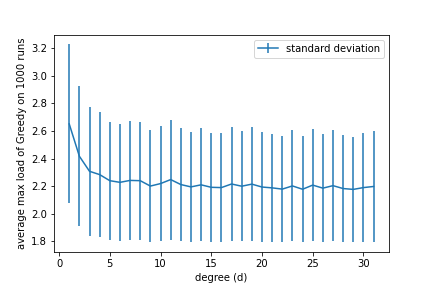
\includegraphics[scale=1.0]{Chapter4/Figs/Greedy_degree_analysis.png}
    \caption{Relating the degree of the graph to the performance of Greedy}
\end{figure}


We can see that indeed smaller degrees hurt Greedy, but after around $d=15$, the performance no longer improves. \NOTE{A}{Why does it perform worse on smaller degree graphs? Give some intuition. Also for why it plateaus. What effect might connectedness have on the performance? Does it matter e.g. for $d=2$ how many components the graph has? Future work...}



Even though Greedy is shown to be suboptimal in some cases, it is still by far the best strategy in the table (apart from DP), it proved to be an impossible challenge for RL to exploit the weaknesses of Greedy. In fact, for $n=m=32$, Deep Q-Learning is not even superior to the Random Strategy, which is equivalent to \textsc{One-Choice} for any regular graph.


\subsection{Deep Q-Learning analysis}

To better understand the difficulty in finding an optimal strategy, I extended the Cycle graph counterexample from Lemma \ref{lemma: greedy-suboptimal} to load vectors of the form $(0, a, 0, b)$, with the edge going between the $2$nd and $3$rd nodes. 


\begin{figure}[h!] \label{greedy-counterexample-analysed}
    \centering
    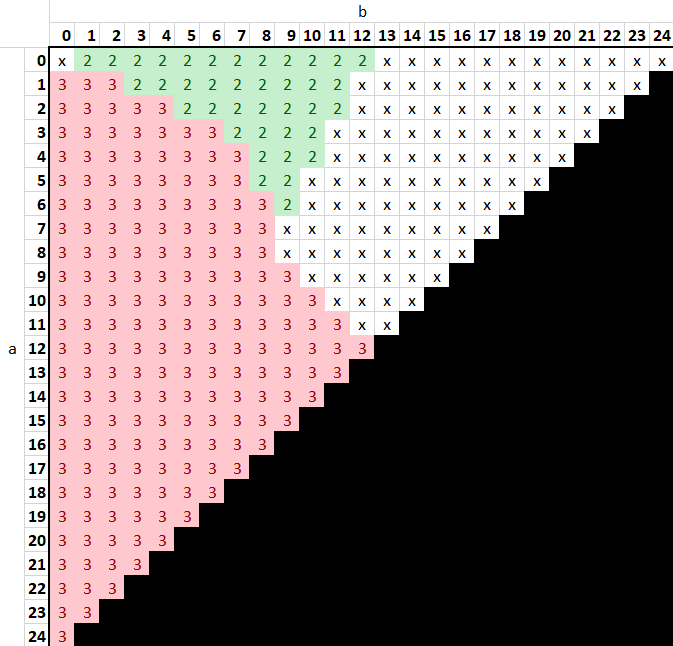
\includegraphics[scale=1.0]{Chapter4/Figs/0a0b_4_25_analysis.png}
    \caption{The optimal decisions for the Cycle graph with $n=4$, $m=25$, load vector $(0,a,0,b)$ and edge $2$-$3$. Green means choosing the $2$nd bin is better, red means choosing the $3$rd bin is better, and $x$ means they have the same expected score.}
\end{figure}


We can see in the figure that the green region contains the counterexamples to the Greedy strategy, but there is an even larger region where the greedy choice is correct, and characterising the shapes of the regions is difficult. By using a neighbourhood average based potential function for Deep Q-Learning, the agent is guided towards choosing $2$rd bin, and by using a graph-oblivious maximum load potential, the agent is guided towards choosing the $3$rd bin. Therefore, neither of the potential functions is perfect. For reference, here are the exact decisions made by the trained Deep Q-Learning strategy: \NOTE{A}{I am not sure if I should include it or not... It doesn't look very promising.}


\begin{figure}[h!] \label{greedy-counterexample-analysed-for-dqn}
    \centering
    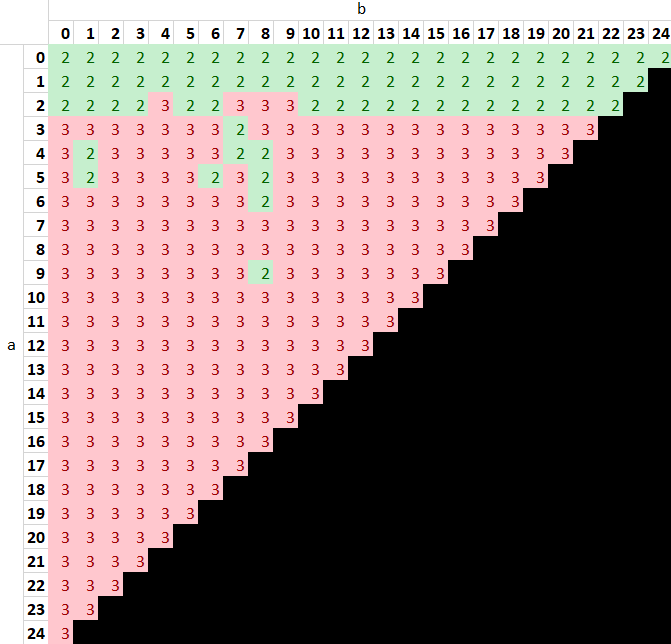
\includegraphics[scale=1.0]{Chapter4/Figs/0a0b_4_25_analysis_dqn.png}
    \caption{The decisions made by the Deep Q-Learning strategy for the Cycle graph with $n=4$, $m=25$, load vector $(0,a,0,b)$ and edge $2$-$3$. Green means choosing the $2$nd bin is better, red means choosing the $3$rd bin is better, and $x$ means they have the same expected score.}
\end{figure}


We can see that the network couldn't learn the exact pattern, though there is some resemblance.


\subsubsection{Training}

I present the training curve for the Hypercube graph with $n=4$ and $m=25$, but the pattern is similar for other cases too.


\begin{figure}[h!] \label{graphical-two-choice-hyperparameter-importance}
    \centering
    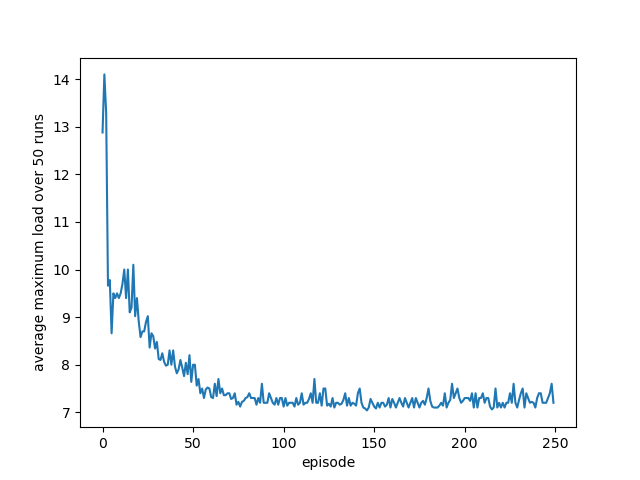
\includegraphics[scale=1.0]{Chapter4/Figs/training_progression_hypercube_4_25.png}
    \caption{\textsc{Graphical Two Choice} Training Curve}
\end{figure}

We can see that unlike for \textsc{Two-Thinning}, the starting point is very poor, so that is a sharp increase initially. After $150$ episodes, the scores plateaus, even though the optimal expected maximum load is even lower.



\subsubsection{Hyperparameter Analysis}

I present the hyperparameter importance analysis of $200$ runs for the Hypercube graph with $n=4$ and $m=25$, but the order is similar for other cases too.

\begin{figure}[h!] \label{graphical-two-choice-hyperparameter-importance}
    \centering
    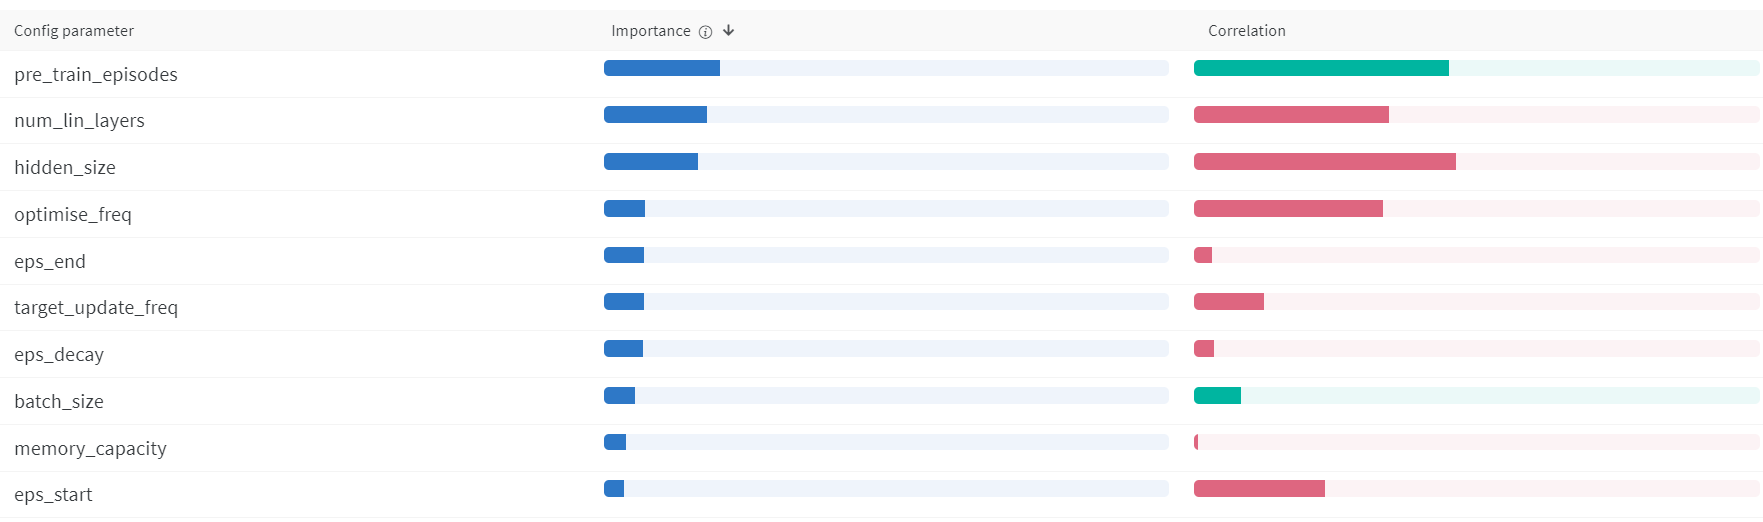
\includegraphics[scale=0.4]{Chapter4/Figs/graphical_two_choice_hypercube_4_25_importance.png}
    \caption{\textsc{Graphical Two Choice} Hyperparameter Importance}
\end{figure}


Unlike the ``use\textunderscore threshold'' parameter for \textsc{Two-Thinning}, there is no very important hyperparameter (in fact, the trained scores are within a $0.4$ range for each analysed combination). The negative correlation of ``hidden\textunderscore size'' and ``num\textunderscore lin\textunderscore layers'' with the score shows that adding complexity to the neural network doesn't help.
